\section{CU2 - Utilisation personnelle}

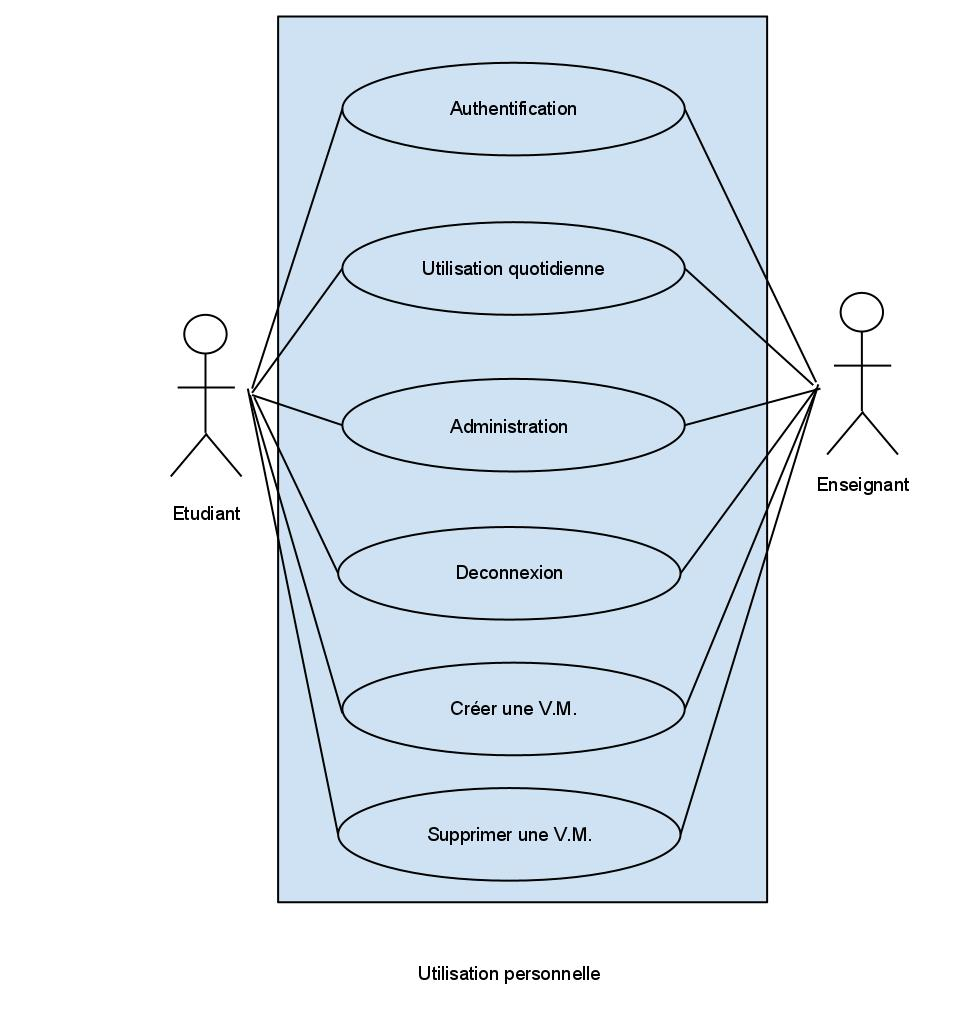
\includegraphics[scale=0.4]{CU2.jpg}

Le but des machines virtuelles est à terme de remplacer le système de session utilisées à l’I.N.S.A.
En terme d’utilisation personnelle, l’enseignant et l’étudiant auraient les mêmes possibilités.

Pour utiliser une machine virtuelle, l’utilisateur (étudiant ou enseignant) devra tout d’abord se connecter (\underline{authentification}). Ensuite, il sera libre d’utiliser sa machine virtuelle afin d’en faire une \underline{utilisation quotidienne} (naviguer sur internet, utiliser des applications, consulter ses e-mails, etc...). Il aura également la possibilité d’effectuer des tâches d’\underline{administration} sur sa machine.

Puisque chaque utilisateur dispose d’un quota pour gérer ses machines virtuelles, il a également la possibilité de créer une nouvelle machine virtuelle (\underline{créer une V.M.}), ou d’en supprimer une existante (\underline{supprimer une V.M.}).

Enfin, l’utilisateur devra enfin lorsqu’il aura cessé d’utiliser une machine virtuelle, utiliser la fonction de \underline{déconnexion}.
